\section{Apéndice 1. Ejemplo de utilización del plugin SERIALIZARDWG.}

\begin{enumerate}

\item{Iniciar la aplicación AutocAD.}

\begin{figure}[H]
\begin{center}
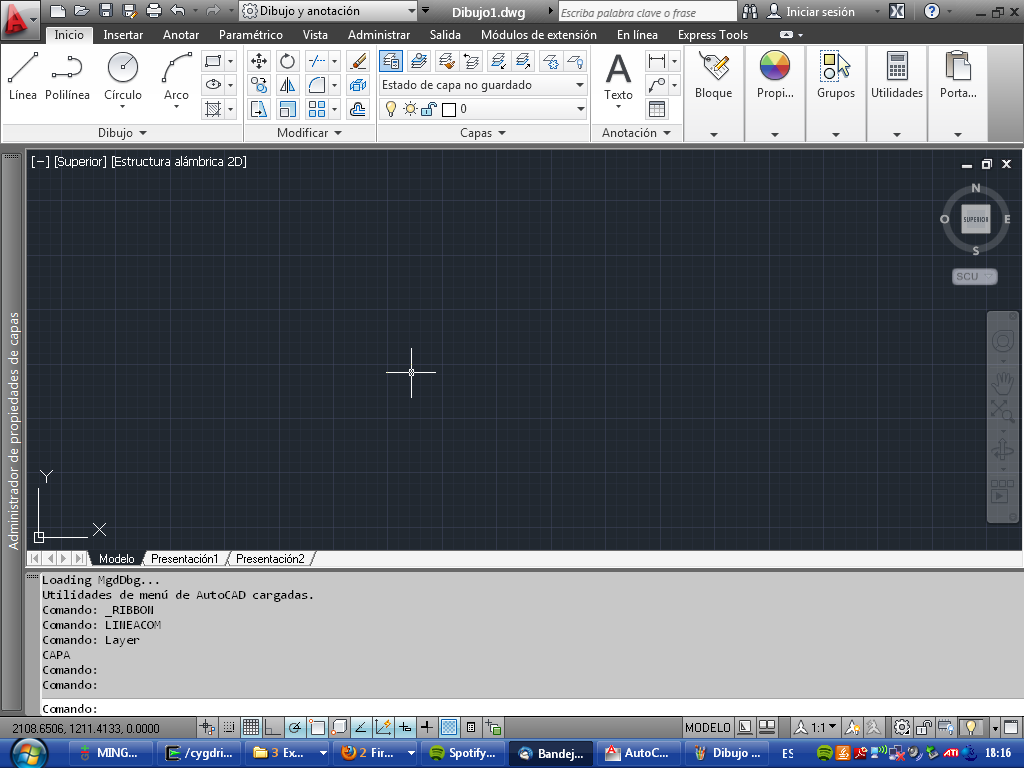
\includegraphics[width=0.65\textwidth]{imgs/autocad0}
\caption{Aplicación AutoCAD.}
\end{center}
\end{figure}

\item{Cargar el plano con la infraestructura que va a ser analizada.}

\begin{figure}[H]
\begin{center}
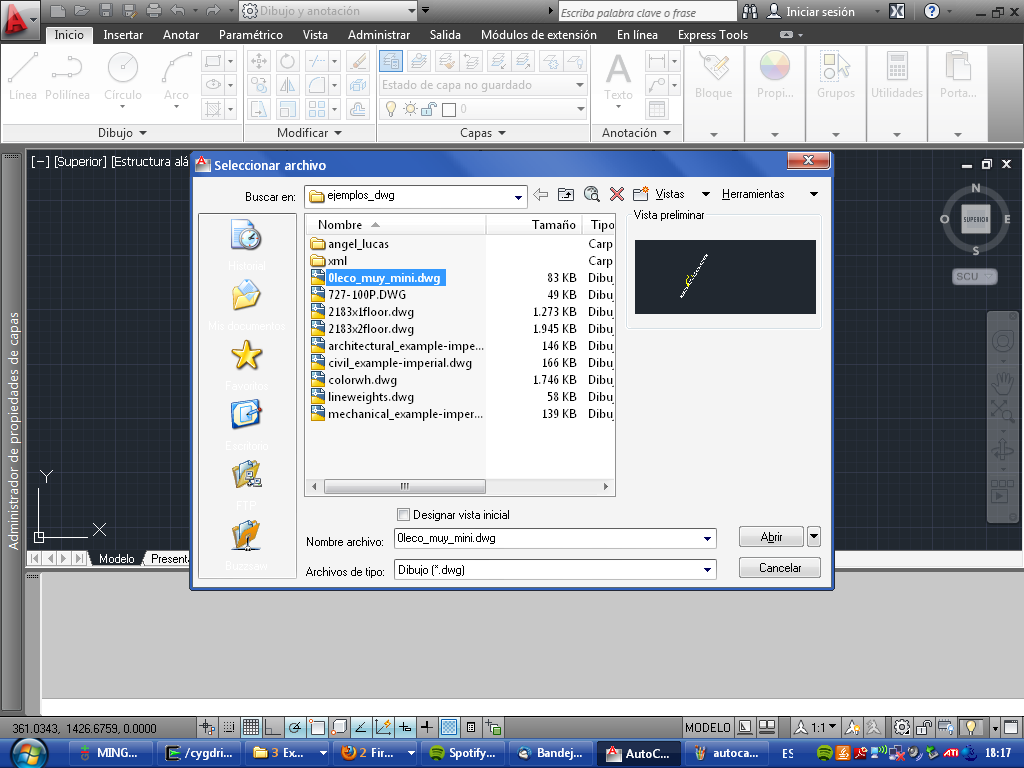
\includegraphics[width=0.65\textwidth]{imgs/autocad1}
\caption{Aplicación AutoCAD abriendo fichero DWG.}
\end{center}
\end{figure}

\begin{figure}[H]
\begin{center}
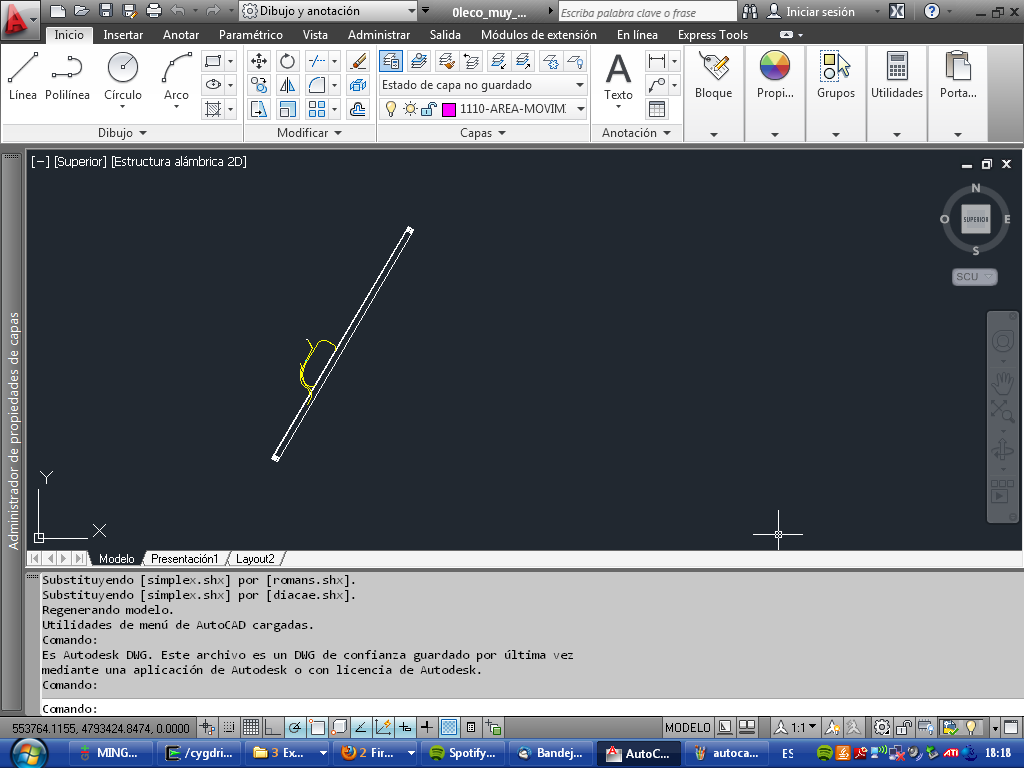
\includegraphics[width=0.65\textwidth]{imgs/autocad2}
\caption{Aplicación AutoCAD mostrando fichero DWG.}
\end{center}
\end{figure}

\item{Cargar el plugin utilizando el comando NETLOAD.}

\begin{figure}[H]
\begin{center}
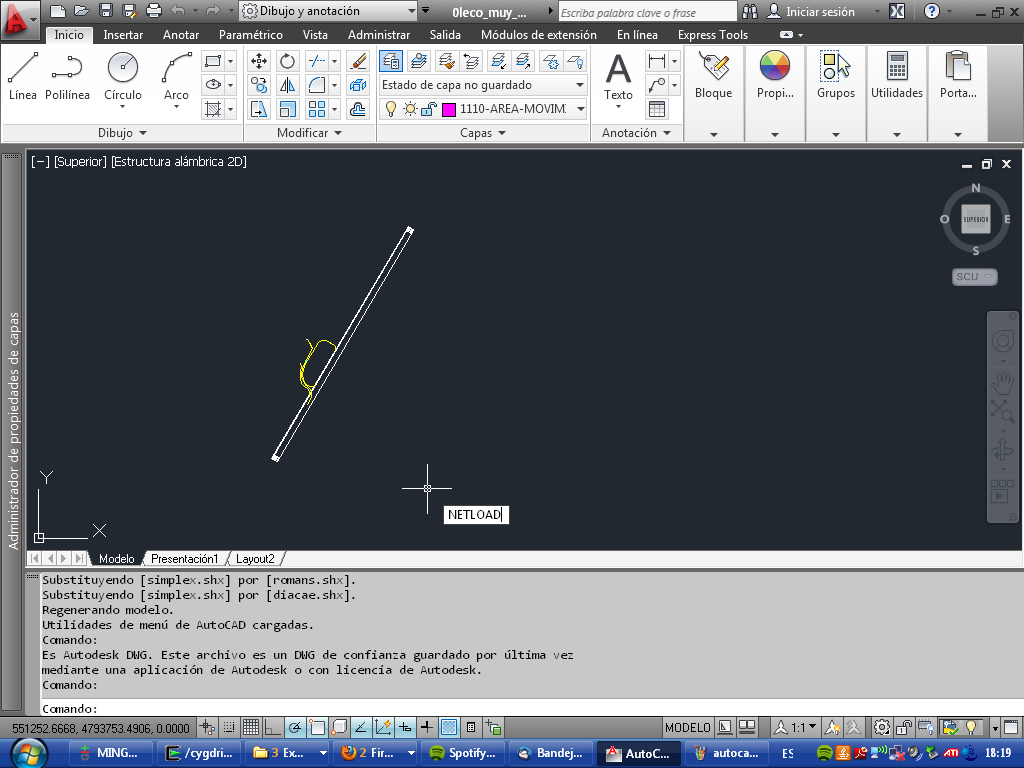
\includegraphics[width=0.65\textwidth]{imgs/autocad3}
\caption{Invocación del comando NETLOAD para cargar el plugin.}
\end{center}
\end{figure}

\item{Seleccionar el fichero DLL que contiene el plugin.}

\begin{figure}[H]
\begin{center}
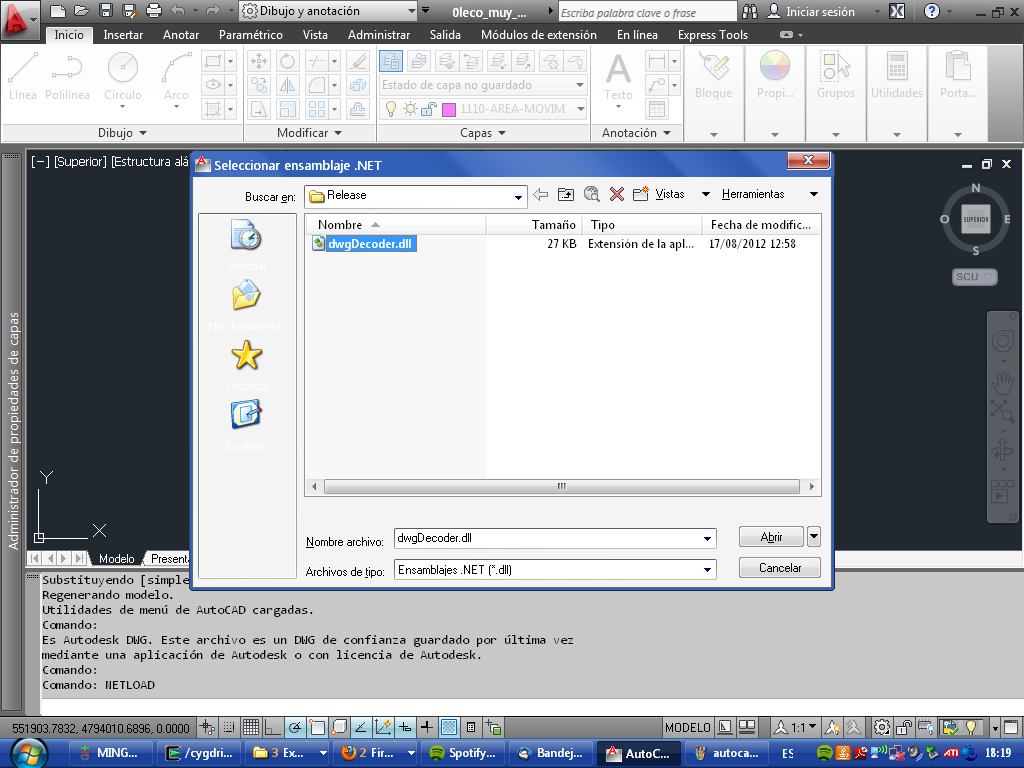
\includegraphics[width=0.65\textwidth]{imgs/autocad4}
\caption{Selección del fichero DLL que contiene el plugin.}
\end{center}
\end{figure}

\item{Lanzar el proceso de extracción con el nuevo comando disponible a través del plugin: SERIALIZARDWG.}

\begin{figure}[H]
\begin{center}
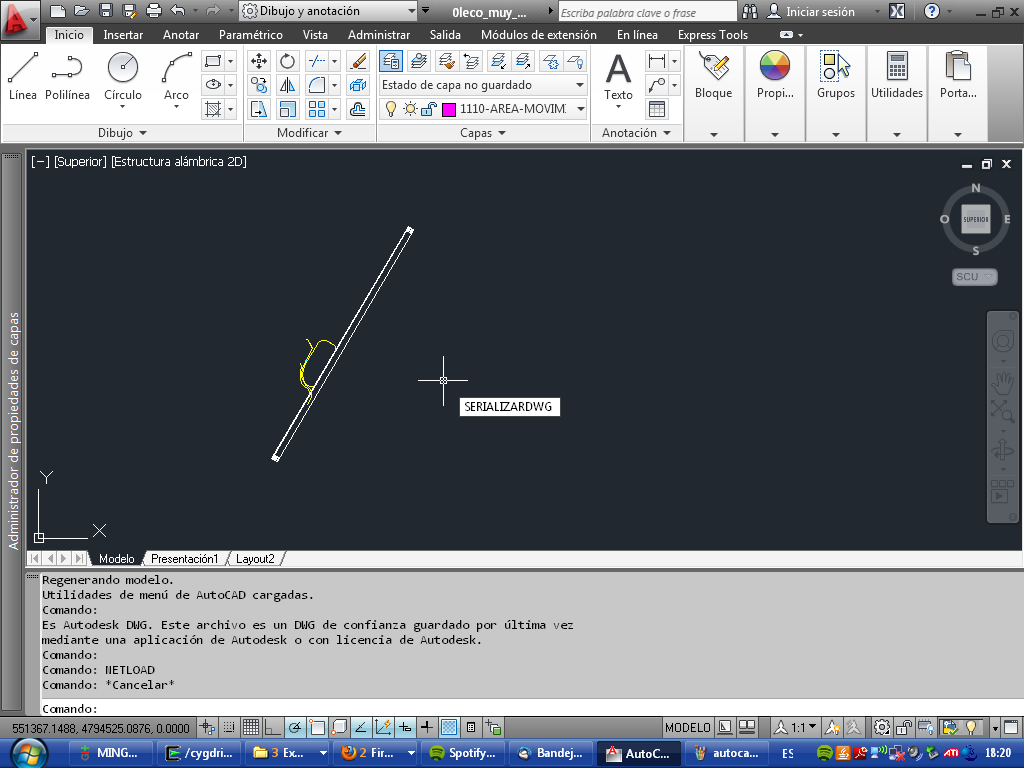
\includegraphics[width=0.65\textwidth]{imgs/autocad5}
\caption{Invocación del comando SERIALIZARDWG implementado en el plugin.}
\end{center}
\end{figure}

\item{Indicar si se desea un log del proceso de extracción.}

\begin{figure}[H]
\begin{center}
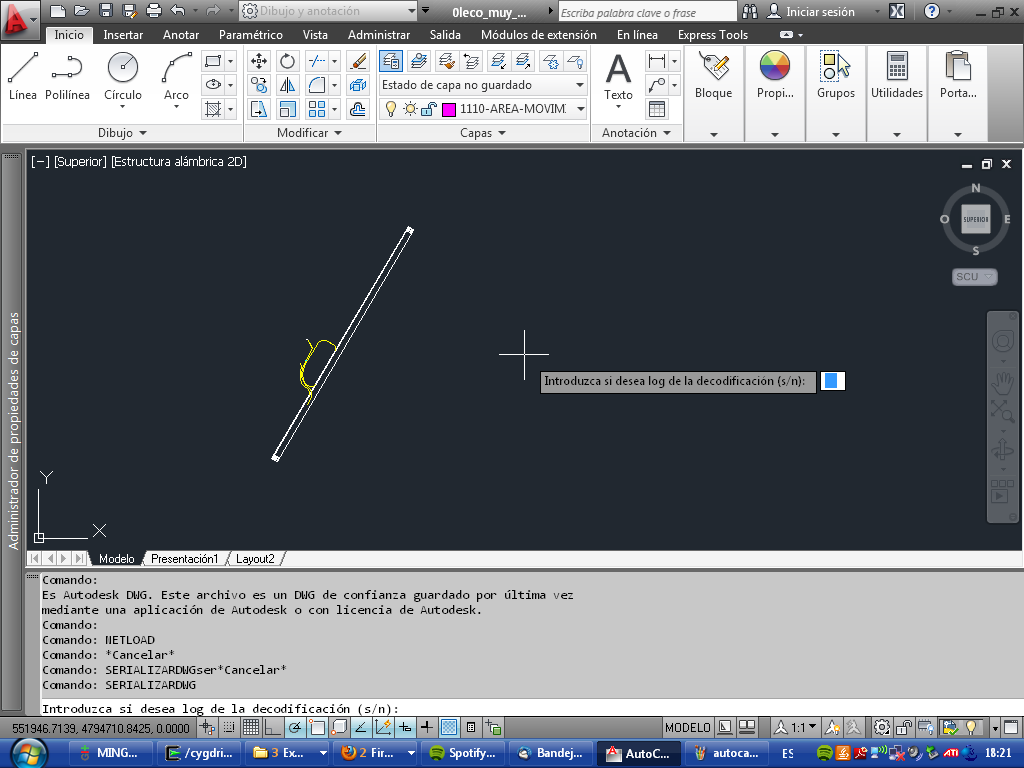
\includegraphics[width=0.65\textwidth]{imgs/autocad6}
\caption{Usuario configurando si desea log del proceso de extracción.}
\end{center}
\end{figure}

\item{Indicar si el log debe incorporar información de depuración. Solo si se ha seleccionado la opción del log.}

\begin{figure}[H]
\begin{center}
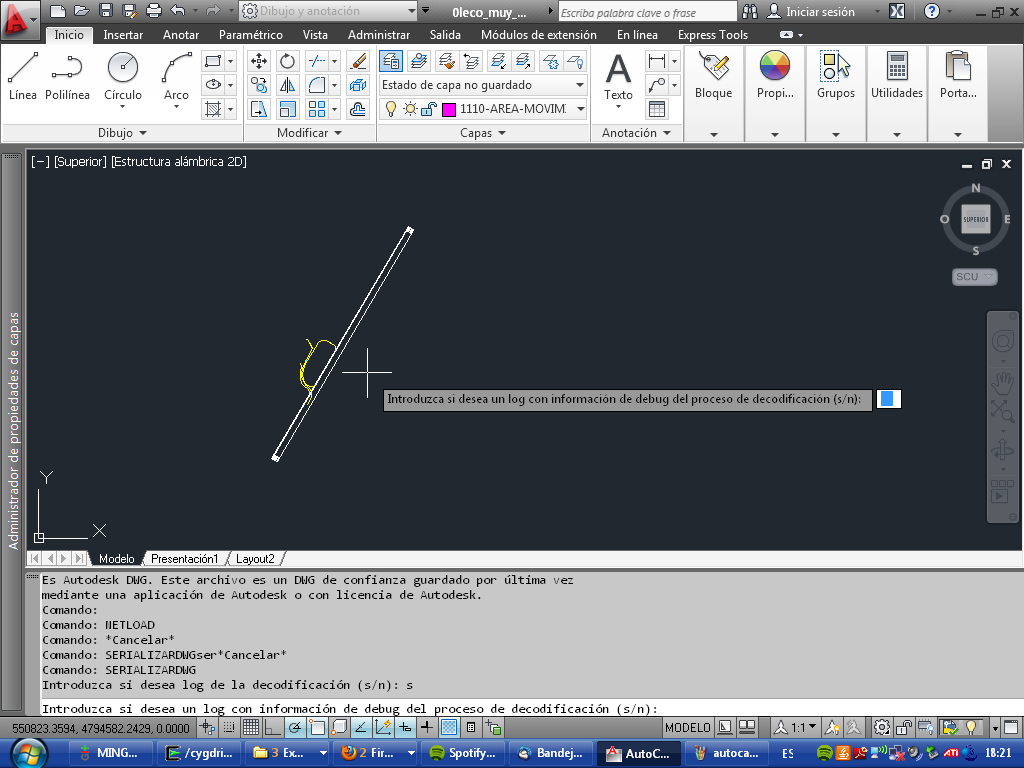
\includegraphics[width=0.65\textwidth]{imgs/autocad7}
\caption{Usuario configurando si desea incorporar información de debug al log del proceso de extracción.}
\end{center}
\end{figure}

\item{Indicar la ruta donde se guardará el fichero con la información extraída del la infraestructura en formato DWG.}

\begin{figure}[H]
\begin{center}
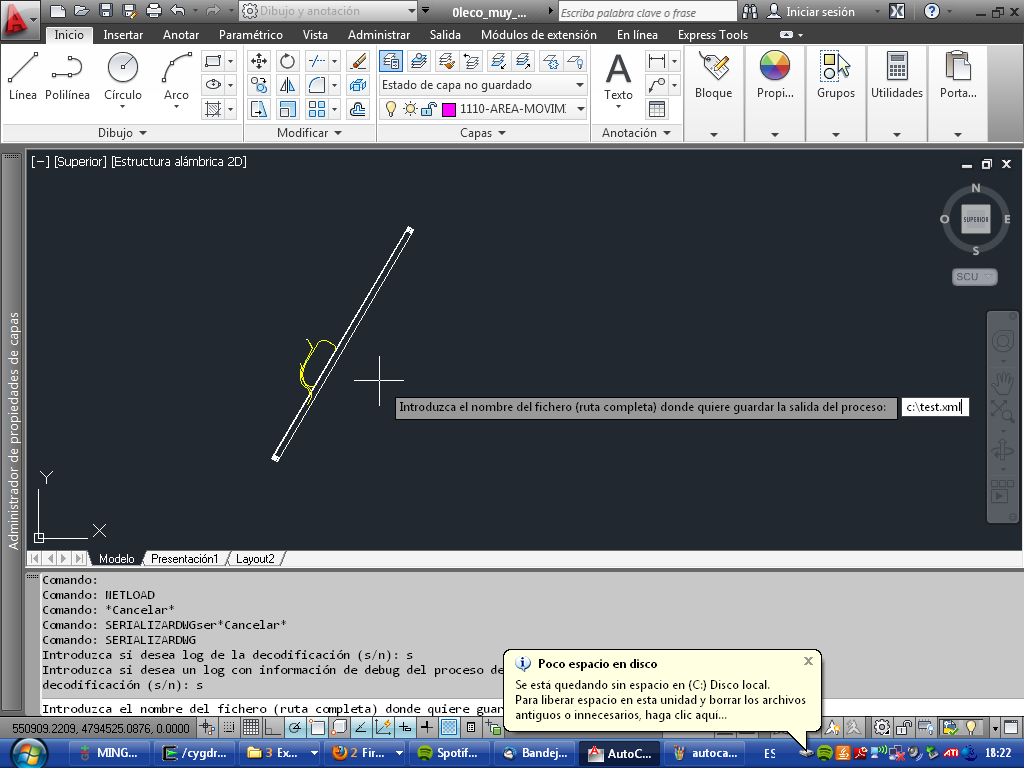
\includegraphics[width=0.65\textwidth]{imgs/autocad8}
\caption{Usuario configurando la ruta donde se almacenará el fichero con la salida del proceso de extracción.}
\end{center}
\end{figure}

\item{Indicar si se desea seleccionar manualmente las capas que deben ser procesadas.}

\begin{figure}[H]
\begin{center}
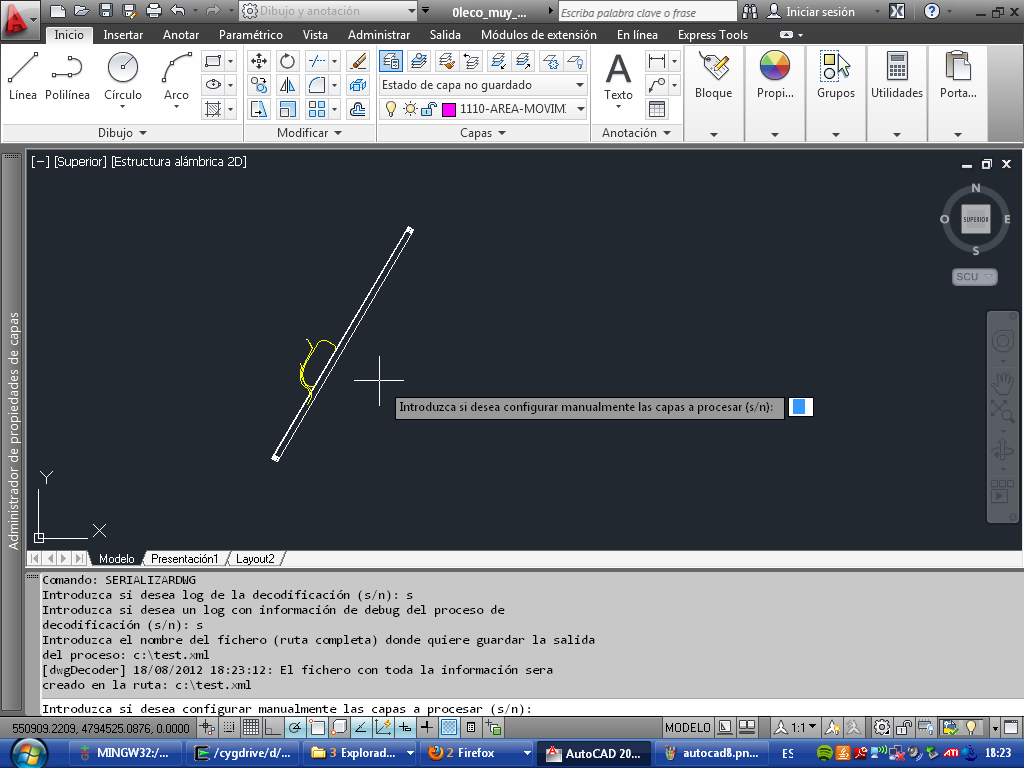
\includegraphics[width=0.65\textwidth]{imgs/autocad9}
\caption{Usuario configurando si desea seleccionar las capas que deben ser procesadas.}
\end{center}
\end{figure}

\item{Indicar capa a capa, según el plugin va solicitándolo, si se desea procesar la capa señalada.}

\begin{figure}[H]
\begin{center}
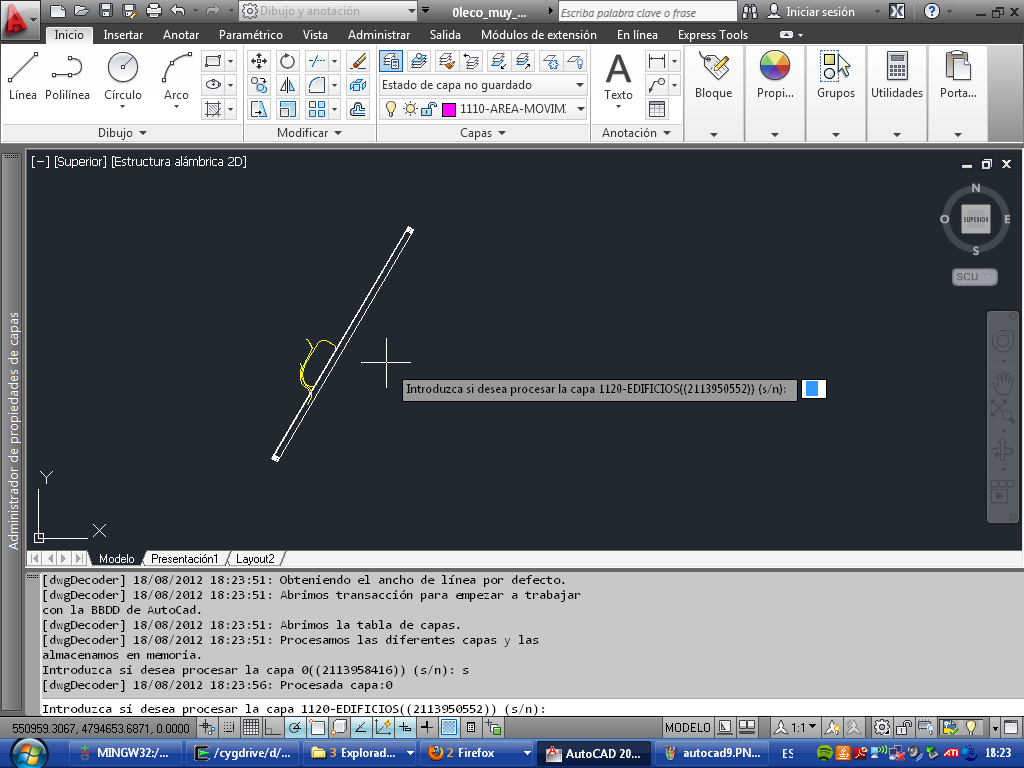
\includegraphics[width=0.65\textwidth]{imgs/autocad10}
\caption{Usuario configurando si desea incluir una capa en el proceso.}
\end{center}
\end{figure}

\item{El proceso de exportación finaliza.}

\begin{figure}[H]
\begin{center}
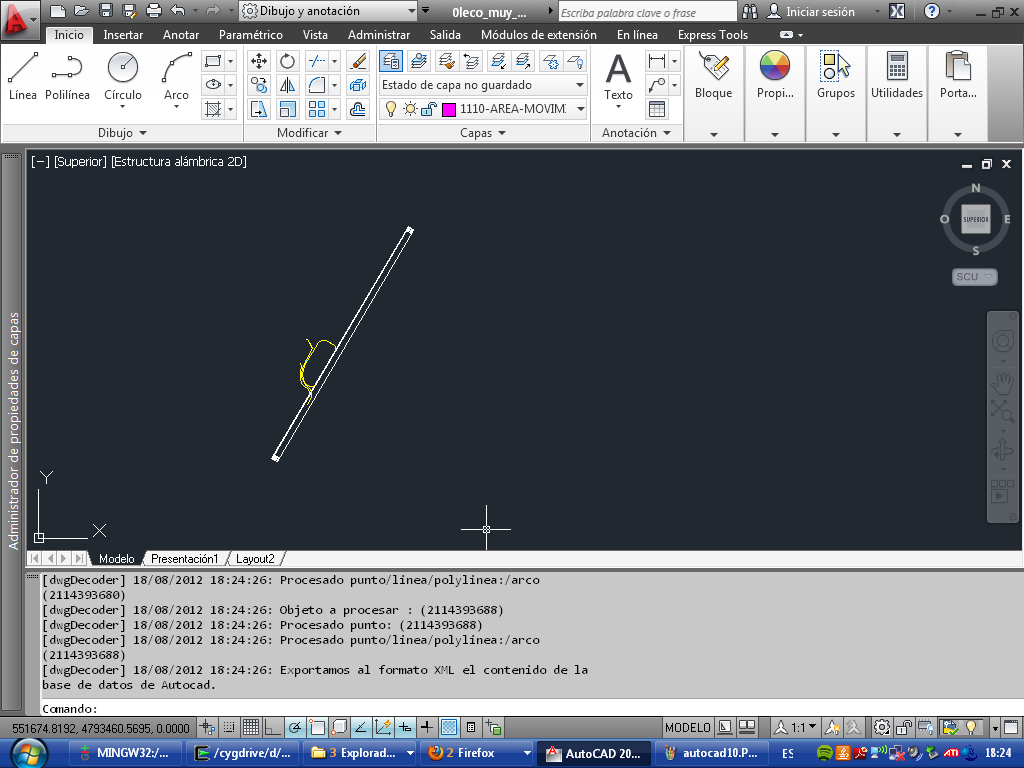
\includegraphics[width=0.65\textwidth]{imgs/autocad11}
\caption{Aplicación AutoCad indicando que la exportación ha finalizado correctamente.}
\end{center}
\end{figure}

\end{enumerate}
